\chapter{Onderhoud en updates}
\chapterpreamble

%
%
%
\section{Firmware flashen}
\label{sec:firmware-flash}

\index{onderhoud}
\index{update}
\index{firmware!flashen}

Het opstarten van de \product gebeurt door middel van het inladen van een programma dat opgeslagen staat op de externe ROM chip van de \sleuf{2} cartridge in het geheugen van de \pkb{P2000T}. Dit programma wordt de firmware genoemd en bevat de benodigde routines om te kunnen communiceren met SD-kaartjes. Deze firmware is continu onderhevig aan verbetering en als eindgebruiker is het wenselijk om de laatste versie met de nieuwste verbeteringen en mogelijkheden te kunnen draaien. Het proces van het updaten of vervangen van de firmware wordt ``flashen'' genoemd. Het flashen van de firmware is betrekkelijk eenvoudig en hiervoor wordt een aparte cartridge ROM geleverd op de \sleuf{1} cartridge.

Om de firmware te flashen dient men de volgende stappen te volgen. 

\begin{enumerate}[noitemsep]
    \item Allereerst moet de laatste versie van de firmware gedownload worden welke te vinden is via onderstaande link:\\
    \url{https://github.com/ifilot/p2000t-sdcard/releases/latest/download/LAUNCHER.BIN}
    \item Plaatst het bestand \pkb{LAUNCHER.BIN} in de \textbf{hoofdmap} op de SD-kaart. Hiervoor heeft u een (USB) SD-kaart lezer op uw desktop computer of laptop nodig.
    \item Stel de DIP switch aan de voorzijde van de \sleuf{1} cartridge\footnote{Zie ook \cref{fig:cartridge-sleuf1}.} zo in dat de \textbf{linkerpin} naar beneden staat en de \textbf{rechterpin} naar boven.
    \item Zet nu de \pkb{P2000T} aan. Op het beeldscherm zal nu een tekst verschijnen vergelijkbaar met \cref{fig:flasher-boot}.
    \item Druk nu op een willekeurige toets om de flash procedure te starten. Allereerst zal de Flasher verbinding proberen te maken met de SD-kaart en vervolgens zoeken of er een bestand met de naam \pkb{LAUNCHER.BIN} in de hoofdmap staat. \index{LAUNCHER.BIN}
    \item Indien dit bestand gevonden wordt, dan zal de cartridge controleren of er een ROM chip in de cartridge zit met een signatuur van \pkb{0xB5BF}, hetgeen overeenkomt met een flash chip van het type \pkb{SST39SF010}.
    \item Vervolgens wordt het geheugen \pkb{0x0000-0x3FFF} op de cartridge ROM chip gewist om plaats te maken voor de nieuwe firmware routines.
    \item Tenslotte wordt de nieuwe firmware overgekopieerd van de SD kaart naar de cartridge ROM chip. Het kopiëren duurt ongeveer een seconde en op het beeldscherm valt een teller te zien.
    \item Na het kopiëren wordt gecontroleerd of de firmware correct is overgezet middels het uitrekenen van een CRC-16 checksum. Deze checksum bevindt zich in de laatste twee bytes van de firmware en heeft een dusdanige waarde dat de gehele CRC-16 checksum uitkomt op \pkb{0x0000}. De laatste twee bytes acteren dus als een soort digitale handtekening. \index{LAUNCHER.BIN!checksum} \index{LAUNCHER.BIN!crc-16} \index{checksum!LAUCHER.BIN} \index{crc-16!LAUNCHER.BIN}
\end{enumerate}

\begin{figure}[h!]
    \centering
    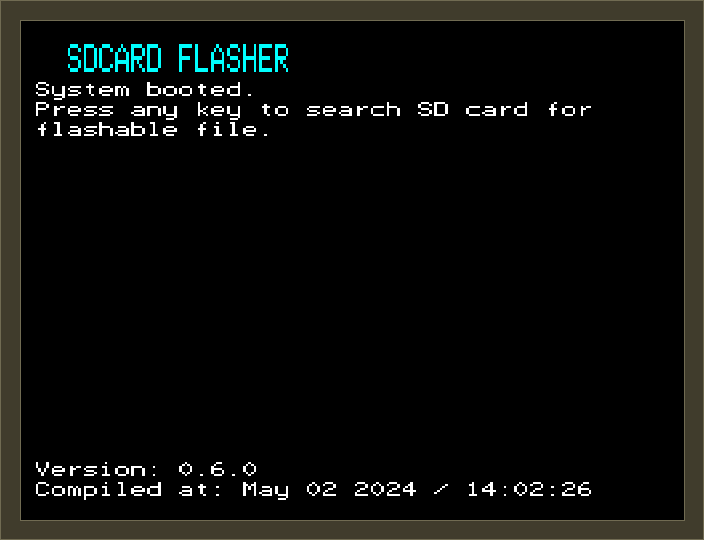
\includegraphics[width=0.99\textwidth]{img/flasher_boot.png}
    \caption{Opstartscherm van de Flasher.}
    \label{fig:flasher-boot}
\end{figure}

Indien alles succesvol is verlopen zal een groene tekst op het beeldscherm verschijnen en ziet men een overzicht van de gehele flashprocedure zoals weergegeven in \cref{fig:flasher-done}.

\index{flashprocedure}

\begin{figure}[h!]
    \centering
    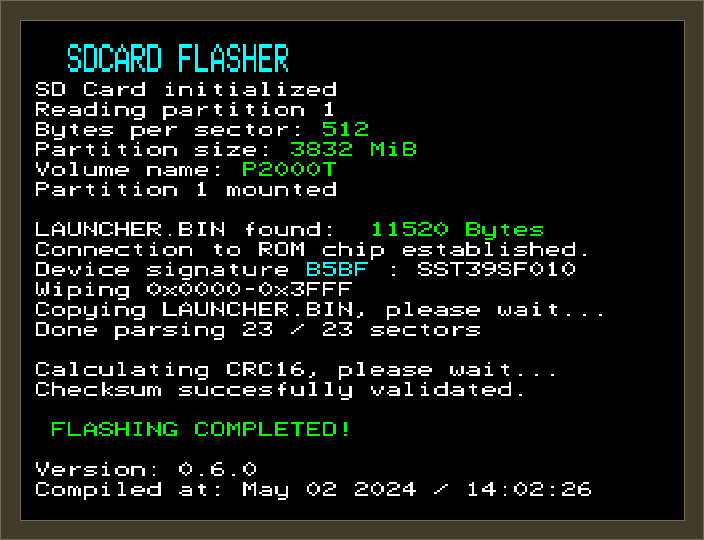
\includegraphics[width=0.99\textwidth]{img/flasher_done.png}
    \caption{Voltooide flash procedure.}
    \label{fig:flasher-done}
\end{figure}

U kunt nu de \pkb{P2000T} uitzetten, de DIP switch op de \sleuf{1} cartridge zo instellen dat beide pinnetjes naar beneden staan en de \pkb{P2000T} opnieuw aanzetten. Het systeem zal dan opstarten met de nieuwe firmware.

%
%
%
\section{Nieuwe bestanden toevoegen}

\index{uploaden|see{toevoegen bestanden}}
\index{toevoegen bestanden}
\index{bestanden!toevoegen aan SD-kaartje}

U kunt nieuwe \cas en \pkb{.PRG} bestanden toevoegen door ze simpelweg naar de SD kaart te kopiëren. Als u veel bestanden op de SD kaart wilt plaatsen is het wenselijk om gebruik te maken van meerdere mappen. Een groot overzicht aan \cas bestanden treft u aan in onderstaande Github repository: \url{https://github.com/p2000t/software/}
onder het mapje ``cassettes''.

\index{cassettes}

Andere bestanden kunt u natuurlijk ook toevoegen aan de SD kaart. Deze zullen getoond worden door de \product, maar u kunt deze bestanden niet opstarten, echter wel inzien. Het kan eventueel nuttig zijn om (zeer) korte tekstbestandjes toe te voegen welke middels \pkb{hexdump} uit te lezen zijn.